%-------------------------------------------------------------------------
% info-S1-classiques.tex
%-------------------------------------------------------------------------

Cette annexe recense quelques algorithmes « historiques » 
dont les principales vertus aujourd'hui sont d'ordre pédagogique.
A ce titre, tout informaticien débutant doit être capable
de les redéfinir lui-même.
Pour simplifier la lecture de ces algorithmes,
ils sont présentés sous forme de fonctions \python\ pour
lesquelles les descriptions, les préconditions et les tests unitaires sont
volontairement omis. 

$$\framebox[8cm]{\begin{minipage}{7.5cm}\footnotesize
{\bf Spécification :}\\
\centerline{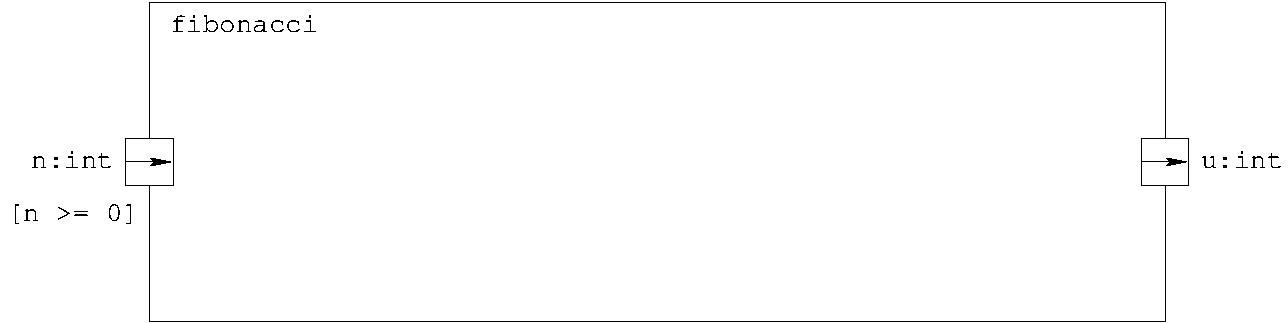
\includegraphics[width=7cm]{fibo-3.pdf}}
$$\begin{minipage}{6.5cm}
{\tt u = fibonacci(n)} est le nombre de Fibonacci à l'ordre {\tt n} si {\tt n:int >= 0}.\\
Exemples : 
\begin{minipage}[t]{3cm}
{\tt fibonacci(0) $\rightarrow$ 1}\\{\tt fibonacci(2) $\rightarrow$ 2}\\{\tt fibonacci(9) $\rightarrow$ 55}
\end{minipage}
\end{minipage}$$

{\bf Implémentation :}\\
\centerline{\includegraphics[width=7cm]{fibo-4.pdf}}
\end{minipage}}$$

%-------------------------------------------------------------------------
%\section*{Algorithme de Bresenham}
%-------------------------------------------------------------------------
%L'algorithme de tracé de segment de Bresenham 
%détermine quels sont les pixels d'un plan discret qui doivent être affichés 
%afin de former une approximation du segment de droite entre deux points donnés.
%$$\includegraphics[width=7cm]{bresenham.jpg}$$

%-------------------------------------------------------------------------
\section*{Algorithme d'Euclide}
%-------------------------------------------------------------------------
\marginpar{\footnotesize\em
\begin{rem}
Voir aussi les exemples \ref{ex:pgcd1} page \pageref{ex:pgcd1},
\ref{ex:pgcd2} page \pageref{ex:pgcd2}, \ref{ex:pgcd3} page \pageref{ex:pgcd3},
la figure \ref{fig:euclide} page \pageref{fig:euclide} et le TD \ref{td:euclide} 
page \pageref {td:euclide}. 
\end{rem}
}
L'algorithme d'Euclide\index{{{\sc Euclide}}} concerne le calcul du plus grand commun diviseur (pgcd) 
de 2 entiers. Le pgcd de 2 entiers $a$ et $b$ peut se calculer en appliquant 
la relation de récurrence ${\rm pgcd}(a,b) = {\rm pgcd}(b,a\%b)$ 
jusqu'à ce que le reste ($a\%b$) soit nul. Cette récurrence se traduit 
par l'algorithme récursif suivant :

\mbox{}\ \ \begin{py}{8cm}
\begin{verbatim}
def pgcd(a,b):
    if b == 0: d = a
    else: d = pgcd(b,a%b)
    return d
\end{verbatim}
\end{py}
\hfill
\begin{py}{5cm}
\begin{verbatim}
>>> pgcd(0,9)
9
>>> pgcd(12,18)
6
\end{verbatim}
\end{py}
\vspace*{2mm}

\noindent L'algorithme ci-dessous est la version itérative de cet algorithme 
récursif.

\index[algo]{algorithme d'{{\sc Euclide}}}
\begin{lstlisting}[caption={\bf Algorithme d'Euclide},label=cl:euclide]
def pgcd(a,b):
    while b != 0:
        r = a % b
        a = b
        b = r	
    return a
\end{lstlisting}

%-------------------------------------------------------------------------
\section*{Coefficients du binôme}
%-------------------------------------------------------------------------
\marginpar{\footnotesize\em
\begin{rem}
Voir aussi les TD \ref{td:iterations} page \pageref{td:iterations} et 
\ref{td:binome} page \pageref{td:binome}.
\end{rem}
\begin{rem} Le coefficient binomial 
$\displaystyle \left(\begin{array}{c}n\\k\end{array}\right)$ 
(ou $\displaystyle C^k_n$, combinaison de $k$ parmi $n$) 
se lit « $k$ parmi $n$ ».
\end{rem}
}
Il s'agit ici de développer le binôme $(a+b)^n$ et de déterminer les coefficients
des termes $a^{n-k}b^k$.
$$(a+b)^n = 
\sum_{k=0}^n \left(\begin{array}{c}n\\k\end{array}\right) a^{n-k}b^k =
\sum_{k=0}^n \frac{n!}{k!(n-k)!}a^{n-k}b^k$$
La formule de Pascal lie les coefficients binomiaux entre eux selon la relation de
récurrence :
$$\left(\begin{array}{c}n\\k\end{array}\right) =
\left(\begin{array}{c}n-1\\k\end{array}\right) +
\left(\begin{array}{c}n-1\\k-1\end{array}\right)
\ \mbox{pour}\ (0 < k < n)\ \mbox{et}\ 
\left(\begin{array}{c}n\\0\end{array}\right) = 
\left(\begin{array}{c}n\\n\end{array}\right) = 1$$
Elle permet un calcul rapide des coefficients pour les petites valeurs de $n$ 
sans division ni multiplication. Elle est utilisée pour construire 
{\em à la main} le triangle de Pascal (remarque \ref{rem:pascal})
et c'est encore elle que est implémentée dans la version récursive 
du calcul des coefficients du binôme.

\mbox{}\ \ \begin{py}{8cm}
\begin{verbatim}
def coefBinome(n,k):
    if k == 0 or n == 0 or n == k: 
        c = 1
    else: 
        c = coefBinome(n-1,k) + coefBinome(n-1,k-1)
    return c
\end{verbatim}
\end{py}
\hfill
\begin{py}{5cm}
\begin{verbatim}
>>> coefBinome(2,1)
1
>>> coefBinome(7,4)
35
>>> coefBinome(14,7)
3432
\end{verbatim}
\end{py}
\vspace*{2mm}

\marginpar{\footnotesize\em
\begin{rem}\label{rem:pascal}Triangle de Pascal\\
\begin{tabular}{l|l}
$n$ & $\displaystyle C^k_n\ (0 \leq k \leq n)$ \\
\hline
0 & \tt 1\\
1 & \tt 1 1\\
2 & \tt 1 2 \ 1\\
3 & \tt 1 3 \ 3 \ 1\\
4 & \tt 1 4 \ 6 \ 4 \ \ 1\\
5 & \tt 1 5 10 10 \ \ 5 \ \ 1\\
6 & \tt 1 6 15 20 \ 15 \ \ 6 \ 1\\
7 & \tt 1 7 21 35 \ 35 \ 21 \ 7 \ 1\\
8 & \tt 1 8 28 56 \ 70 \ 56 28 \ 8 \ 1\\
9 & \tt 1 9 36 84 126 126 84 36 \ 9 \ 1\\
$\vdots$ & $\vdots$
\end{tabular}
\end{rem}}
\noindent La version itérative ci-dessous calcule directement le
numérateur {\tt num} et le dénominateur {\tt den} du coefficient 
{\tt c} en tenant compte de la simplification suivante :
$$\left(\begin{array}{c}n\\k\end{array}\right) = 
\frac{n!}{k!(n-k)!} = 
\frac{n\cdot(n-1)\cdots(n-k+2)\cdot(n-k+1)}{1\cdot2\cdot3\cdots k}$$

\index[algo]{coefficients du binôme}
\begin{lstlisting}[caption={\bf Coefficients du binôme},label=cl:binome]
def coefBinome(n,k):
    num, den = 1, 1
    for i in range(1,k+1):
        num = num*(n-i+1)
        den = den*i
    c = num/den
    return c
\end{lstlisting}


%-------------------------------------------------------------------------
\section*{Conversion en base $b$}
%-------------------------------------------------------------------------
\mbox{}\marginpar{\footnotesize\em
\begin{rem}
Voir aussi l'exemple \ref{ex:numeration} page \pageref{ex:numeration} et les
TD \ref{td:codageEntier} page \pageref{td:codageEntier},
\ref{td:decoder} page \pageref{td:decoder} et
\ref{td:codage} page \pageref{td:codage}.
\end{rem}}
Un entier $n$ en base $b$ est représenté par une suite de
chiffres {$(r_mr_{m-1}\ldots r_1r_0)_b$}
où les $r_i$ sont des chiffres de la base $b$ ($0\leq r_i < b$).
Ce nombre $n$ a pour valeur $\displaystyle\sum^{i=m}_{i = 0} r_ib^i$.
$$n = r_mb^m + r_{m-1}b^{m-1} + \ldots + r_1b^1 + r_0b^0 = 
\sum^{i=m}_{i = 0} r_ib^i$$

Nous choisirons ici de représenter un tel nombre
par une liste {\tt [}$r_m,r_{m-1},\ldots,r_1,r_0${\tt ]}.
L'algorithme de conversion consiste à diviser successivement 
le nombre $n$ par la base $b$ ($n = bq + r$) tant que le quotient $q$ n'est pas nul.
L'ordre inverse des restes des différentes divisions
(du dernier au premier reste, écrits de gauche à droite)
donne la représentation du nombre $n$ en base $b$.
$$\begin{tabular}{lp{5cm}}
$\displaystyle\begin{array}{lll}
n &=& q_0b + r_0 = q_0b^1 + {r_0b^0}\\
n &=& (q_1b^1 + r_1)b^1 + r_0b^0 = q_1b^2 + {r_1b^1 + r_0b^0} \\
n &=& (q_2b^1 + r_2)b^2 + r_1b^1 + r_0b^0 = 
	q_2b^3 + {r_2b^2 + r_1b^1 + r_0b^0}\\
n &=& \ldots\\
n &=& {0}\cdot b^{m+1} + {r_mb^m + \ldots + r_2b^2 + r_1b^1 + r_0b^0} = 
	\displaystyle{\sum^{i=m}_{i = 0} r_ib^i}\\
n  &=& {(r_mr_{m-1}\ldots r_1r_0)_b}
\end{array}$
&
\begin{minipage}{4.5cm}
\footnotesize\tt
\mbox{}>>> conversion(23,10)\newline
\mbox{}[2, 3]\newline
\mbox{}>>> conversion(23,2)\newline
\mbox{}[1, 1, 1, 0, 1]\newline
\mbox{}>>> conversion(23,5)\newline
\mbox{}[3, 4]\newline
\mbox{}>>> conversion(23,12)\newline
\mbox{}[1, 11]\newline
\mbox{}>>> conversion(23,16)\newline
\mbox{}[1, 7]\newline
\end{minipage}
\end{tabular}
$$

\index[algo]{codage en base $b$}
\begin{lstlisting}[caption={\bf Conversion en base $b$},label=cl:conversion]
def conversion(n,b):
    code = []
    if n == 0:
        code = [0]
    while n != 0:
        code.insert(0,n%b)
        n = n/b
    return code
\end{lstlisting}


%-------------------------------------------------------------------------
\section*{Courbe fractale de Koch}
%-------------------------------------------------------------------------
\marginpar{\footnotesize\em
\begin{rem}
Voir aussi le TD \ref{td:fractal} page \pageref{td:fractal}.
\end{rem}
}

La courbe de von Koch \index{{{\sc Von Koch}}} est l'une des premières courbes 
fractales à avoir été décrite par le mathématicien suédois Helge von Koch (1870-1924).
On peut la créer à partir d'un segment de droite, en modifiant récursivement 
chaque segment de droite de la façon suivante :
\begin{enumerate}
\item on divise le segment de droite en trois segments de longueurs égales,
\item on construit un triangle équilatéral ayant pour base le segment médian 
	de la première étape,
\item on supprime le segment de droite qui était la base du triangle 
	de la deuxième étape.
\end{enumerate}
Avec les instructions {\em à la {\sc Logo}} (voir annexe \ref{logo}
page \pageref{logo}), on obtient l'algorithme récursif ci-dessous
pour dessiner de telles courbes (figure \ref{fig:koch2}).

\marginpar{\footnotesize\em
\fbox{\begin{minipage}{8cm}\label{fig:koch2}
Courbes de von Kock pour $n=0$ (courbe du bas),
$n=1$ (courbe du milieu) et $n=2$ (courbe du haut).
$$\includegraphics[width=7.5cm]{vonkock.jpg}$$
Les flocons de Koch s'obtiennent de la même façon que les courbes fractales, 
en partant d'un polygone régulier au lieu d'un segment de droite.\\
Ci-dessous, les flocons heptagonaux pour $n=0$ (flocon de gauche),
$n=1$ (flocon du milieu) et $n=2$ (flocon de droite).
$$\includegraphics[width=7.5cm]{flocon2.jpg}$$
\end{minipage}}
}
\index[algo]{courbes fractales}
\begin{lstlisting}[caption={\bf Courbe fractale de Koch},label=cl:fractal]
def kock(n,d):
    if n == 0: forward(d)
    else:
        kock(n-1,d/3.)
        left(60)
        kock(n-1,d/3.)
        right(120)
        kock(n-1,d/3.)
        left(60)
        kock(n-1,d/3.)
    return
\end{lstlisting}

%-------------------------------------------------------------------------
\section*{Crible d'Eratosthène}
%-------------------------------------------------------------------------
Le crible d'Ératosthène (mathématicien grec du $3^{\grave eme}$ siècle avant JC)\index{{{\sc Eratosthène}}}
est un algorithme pour trouver tous les nombres premiers inférieurs à 
un certain entier naturel donné $n$.
On forme une liste avec tous les entiers naturels compris entre 2 et $n$ 
({\tt range(2,n+1)}) et on supprime les uns après les autres, 
les entiers qui ne sont pas premiers de la manière suivante : 
on commence par le début de la liste et dès que l'on trouve un entier 
qui n'a pas encore été supprimé, il est déclaré premier, on le supprime
ainsi que tous les autres multiples de celui-ci et on recommence tant que
la liste n'est pas vide. L'algorithme récursif suivant le généralise
à toutes listes, triées par ordre croissant, d'entiers supérieurs ou égaux à 2.

\mbox{}\ \ \begin{py}{8cm}
\begin{verbatim}
def crible(t):
    if t[0]**2 > t[-1]: premiers = t
    else:
        premiers = []
        for element in t:
            if element%t[0] != 0:
                premiers.append(element)
        premiers = t[:1] + crible(premiers)
    return premiers
\end{verbatim}
\end{py}
\hfill
\begin{py}{5cm}
\begin{verbatim}
>>> crible(range(2,14))
[2, 3, 5, 7, 11, 13]
>>> crible(range(2,100))
[2, 3, 5, 7, 11, 13, 17, 19, 23,
 29, 31, 37, 41, 43, 47, 53, 59, 
 61, 67, 71, 73, 79, 83, 89, 97] 
>>> crible(range(2,14,3))
[2, 5, 11]
\end{verbatim}
\end{py}
\vspace*{2mm}

\noindent Un algorithme itératif correspondant est présenté ci-dessous.

\index[algo]{crible d'{{\sc Eratosthène}}}
\index[algo]{nombres premiers|see{crible d'{{\sc Eratosthène}}}}
\begin{lstlisting}[caption={\bf Crible d'Eratostène},label=cl:eratostene]
def crible(t):
    i = 0
    while i < len(t):
        j = i+1
        while j < len(t):
            if t[j]%t[0] == 0: del t[j]
            else: j = j + 1
        i = i + 1    
    return t
\end{lstlisting}

%-------------------------------------------------------------------------
\section*{Développement limité de la fonction $\sin(x)$}
%-------------------------------------------------------------------------
\marginpar{\footnotesize\em
\begin{rem}
Voir aussi l'exemple \ref{ex:exp} page \pageref{ex:exp}
et les TD \ref{td:sinus} page \pageref{td:sinus} et 
\ref{td:dev} page \pageref{td:dev}.
\end{rem}
}
Les développements limités des fonctions usuelles s'écrivent sous la forme 
de développements en série entière $\displaystyle \sum_{k=0}^{n} u_k$ comme
par exemple pour la fonction sinus :
$$\sin(x) \approx \sum_{k=0}^{n} u_k = \sum_{k=0}^{n} (-1)^k\frac{x^{2k+1}}{(2k+1)!}\\
\mbox{}\hfill = x - \frac{x^3}{6} + \frac{x^5}{120} + \ldots + (-1)^n\frac{x^{2n+1}}{(2n+1)!}$$
Ces développements font souvent intervenir les fonctions puissance et
factorielle qui sont très «~gourmandes~» en temps de calcul; 
on cherche alors à éviter leur utilisation en s'appuyant sur une relation 
de récurrence entre les $u_k$. Ainsi, pour la fonction sinus :
$$u_{k+1} = (-1)^{k+1}\frac{x^{2(k+1)+1}}{(2(k+1)+1)!} = -(-1)^k\frac{x^{2k+1}}{(2k+1)!}\frac{x^2}{(2k+2)(2k+3)} =
-u_k\frac{x^2}{(2k+2)(2k+3)}$$
Ce qui conduit à l'algorithme itératif ci-dessous.

\index[algo]{développements limités}
\begin{lstlisting}[caption={\bf Développement limité},label=cl:developpement]
def sinus(x,n):
    u = x
    y = u
    for k in range(0,n+1):
        u = -((x*x)/((2*k+2)*(2*k+3)))*u
        y = y + u
    return y
\end{lstlisting}
\marginpar{\footnotesize\em
\begin{rem}Rappels:\\
$$\sin(\frac{\pi}{6}) = \frac{1}{2}\hspace*{5mm}
\sin(\frac{\pi}{2}) = 1\hspace*{5mm}
\sin(\pi) = 0$$
\end{rem}
}

\mbox{}\ \ \begin{py}{4cm}
\begin{verbatim}
>>> sinus(pi/6,3)
0.50000000002027989
>>> sinus(pi/2,3)
1.0000035425842861
>>> sinus(pi,3)
0.0069252707075050518
\end{verbatim}
\end{py}
\hfill
\begin{py}{4cm}
\begin{verbatim}
>>> sinus(pi/6,7)
0.49999999999999994
>>> sinus(pi/2,7)
1.0000000000000437
>>> sinus(pi,7)
2.2419510632012503e-08
\end{verbatim}
\end{py}
\hfill
\begin{py}{4cm}
\begin{verbatim}
>>> sinus(pi/6,70)
0.49999999999999994
>>> sinus(pi/2,70)
1.0000000000000002
>>> sinus(pi,70)
2.4790606856821868e-16
\end{verbatim}
\end{py}
\vspace*{2mm}

%-------------------------------------------------------------------------
\section*{Fonction factorielle}
%-------------------------------------------------------------------------
\marginpar{\footnotesize\em
\begin{rem}
Voir aussi l'exemple \ref{ex:factorielle} page \pageref{ex:factorielle}
et les TD \ref{td:factorielle} page \pageref{td:factorielle} et 
\ref{td:traceFactorielle} page \pageref{td:traceFactorielle}.
\end{rem}
}

La fonction factorielle qui calcule le produit des 
$n$ premiers entiers positifs  
est simplement définie par la relation de
récurrence :
$$\left\{\begin{array}{l@{\ =\ }ll}
0! & 1 & \\
n! & n\cdot (n-1)! & \forall n \in N^*
\end{array}\right.\hspace*{1cm}
\left(n! = \prod_{k=1}^n k\right)$$
Cette relation de récurrence est implémentée de manière récursive
de la manière suivante :

\mbox{}\ \ \begin{py}{8cm}
\begin{verbatim}
def factorielle(n):
    if n < 2: u = 1
    else: u = n * factorielle(n-1)
    return u
\end{verbatim}
\end{py}
\hfill
\begin{py}{5cm}
\begin{verbatim}
>>> factorielle(0)
1
>>> factorielle(5)
120
>>> factorielle(10)
3628800
\end{verbatim}
\end{py}
\vspace*{2mm}

\noindent L'algorithme itératif du calcul de $n!$ est donné ci-dessous.

\index[algo]{fonction factorielle}
\begin{lstlisting}[caption={\bf Fonction factorielle},label=cl:factorielle]
def factorielle(n):
    u = 1
    for i in range(2,n+1):
       u = u * i
    return u
\end{lstlisting}

%-------------------------------------------------------------------------
\section*{Fonction puissance}
%-------------------------------------------------------------------------
\marginpar{\footnotesize\em
\begin{rem}
Voir aussi l'exemple \ref{ex:puissance} page \pageref{ex:puissance}
et le TD \ref{td:puissance} page \pageref{td:puissance}.
\end{rem}
}
La puissance entière $p$ d'un nombre $x$ est définie par :
$\displaystyle p = x^n = \prod_{k=1}^{n} x = \underbrace{x\cdot x\cdot x\cdots x}_{n\ \rm fois}$ .
On peut la définir de manière récursive comme ci-dessous :

\mbox{}\ \ \begin{py}{8cm}
\begin{verbatim}
def puissance(x,n):
    if n == 0: p = 1
    else: p = x * puissance(x,n-1)
    return p
\end{verbatim}
\end{py}
\hfill
\begin{py}{5cm}
\begin{verbatim}
>>> puissance(2,0)
1
>>> puissance(2,20)
1048576
\end{verbatim}
\end{py}
\vspace*{2mm}

\noindent L'algorithme itératif du calcul de $x^n$ est le suivant.

\index[algo]{fonction puissance}
\begin{lstlisting}[caption={\bf Fonction puissance},label=cl:puissance]
def puissance(x,n):
    p = x
    for k in range(1,n):
        p = p*x
    return p
\end{lstlisting}

%-------------------------------------------------------------------------
\section*{Nombres de Fibonacci}
%-------------------------------------------------------------------------
\marginpar{\footnotesize\em
\begin{rem}
Voir aussi l'exemple \ref{ex:fibonacci} page \pageref{ex:fibonacci},
les figures \ref{fig:fibo3} page \pageref{fig:fibo3} et \ref{fig:recursivite} 
page \pageref{fig:recursivite} et
la remarque \ref{rem:fibonacci} page \pageref{rem:fibonacci}.
\end{rem}
}
Les nombres de Fibonacci sont donnés par la suite définie par la relation de récurrence ci-dessous :
$$ \left\{\begin{array}{l}
f_0 = f_1 = 1\\
f_n = f_{n-1} + f_{n-2}\ \forall n > 1
\end{array}\right.$$
Les 10 premiers nombres de la suite de Fibonacci valent donc
successivement $f_0 = 1$, $f_1 = 1$, $f_2 = 2$, $f_3 = 3$, 
$f_4 = 5$, $f_5 = 8$, $f_6 = 13$, $f_7 = 21$, $f_8 = 34$, et $f_9 = 55$.

Le $n^{\grave eme}$ nombre de Fibonacci peut donc se calculer de manière récursive en 
appliquant simplement la définition de la suite de Fibonacci.

\mbox{}\ \ \begin{py}{8cm}
\begin{verbatim}
def fibonacci(n):
    if n < 2: f = 1
    else: f = fibonacci(n-1) + fibonacci(n-2)
    return f
\end{verbatim}
\end{py}
\hfill
\begin{py}{5cm}
\begin{verbatim}
>>> for n in range(0,10): 
        print fibonacci(n),

1 1 2 3 5 8 13 21 34 55
\end{verbatim}
\end{py}
\vspace*{2mm}

%\newpage
\noindent Un algorithme itératif du calcul du $n^{\grave eme}$ nombre de 
Fibonacci est présenté ci-dessous.

\index[algo]{nombres de {{\sc Fibonacci}}}
\begin{lstlisting}[caption={\bf Nombres de Fibonacci},label=cl:fibonacci]
def fibonacci(n):
    f,f1,f2 = 2,1,1
    for i in range(3,n+1) :
        f2 = f1
        f1 = f
        f = f1 + f2
    return f
\end{lstlisting}

%-------------------------------------------------------------------------
\section*{Palindrome}
%-------------------------------------------------------------------------
Un palindrome est une séquence dont l'ordre des éléments reste le même 
qu'on la parcourt du premier au dernier ou du dernier au premier.
Ainsi, {\tt [1,2,2,1]}, {\tt "kayak"} sont des palindromes au même
titre que l'expression arithmétique {\tt 1234+8765=9999=5678+4321}.
Dans les chaînes de caractères, si l'on ne prend pas en compte la casse 
(minuscules ou majuscules), les espaces, les signes de ponctuation
et les signes diacritiques (accents, cédilles), alors 
{\tt "engage le jeu que je le gagne"} et {\tt "A man, a plan, a canal: Panama"} 
sont également des palindromes.

\newpage
\index[algo]{palindrome}
\begin{lstlisting}[caption={\bf Palindrome},label=cl:palindrome]
def palindrome(t):
    n, i, ok = len(t), 0, True
    while i < n/2 and ok == True:
        if t[i] != t[n-1-i]: ok = False
	else: i = i + 1
    return ok      
\end{lstlisting}

%-------------------------------------------------------------------------
\section*{Produit de matrices}
%-------------------------------------------------------------------------
\marginpar{\footnotesize\em
\begin{rem}
Voir aussi le TD \ref{td:matrices1} page \pageref{td:matrices1}. 
\end{rem}

\begin{rem}
Le produit de deux matrices n'est défini que si le nombre $r$ de colonnes 
de la première matrice est égal au nombre de lignes de la deuxième 
matrice.
\end{rem}
}

Le produit $C$ de 2 matrices $A$ et $B$ respectivement de dimensions 
$(n,r)$ et $(r,m)$ est tel que :
$$c_{i,j} = \sum_{k=0}^{r-1}a_{ik}\cdot b_{kj}$$

\index[algo]{produit de matrices}
\begin{lstlisting}[caption={\bf Produit de matrices},label=cl:produitMatrices]
def produitMatrice(a,b):
    c = []
    n,r,m = len(a),len(a[0]),len(b[0])
    for i in range(n):
        c.append([])
        for j in range(m):
            x = 0
            for k in range(r):
                x = x + a[i][k]*b[k][j]
            c[i].append(x)
    return c
\end{lstlisting}

\mbox{}\ \ \begin{py}{8cm}
\begin{verbatim}
>>> a = [[1,2],[3,4]]
>>> b = [[2,1],[-1,-2]]
>>> produitMatrice(a,b)
[[0, -3], [2, -5]]
\end{verbatim}
\end{py}
\hfill
\begin{py}{5cm}
\begin{verbatim}
>>> a = [[1,2,3,4]]
>>> b = [[1],[2],[3],[4]]
>>> produitMatrice(a,b)
[[30]]
\end{verbatim}
\end{py}


%-------------------------------------------------------------------------
\section*{Recherche dichotomique}
%-------------------------------------------------------------------------
\marginpar{\footnotesize\em
\begin{rem}
Voir aussi la section \ref{sub:rechercheDichotomique} page \pageref{sub:rechercheDichotomique} 
consacrée à la recherche dichotomique.
\end{rem}
}
Il s'agit d'un algorithme de recherche d'un élément {\tt x} dans une liste {\tt t} déjà triée.
\index{recherche dans une séquence!recherche dichotomique}
Le principe de la recherche dichotomique consiste à comparer {\tt x} avec l'élément
{\tt t[m]} du milieu de la liste {\tt t} triée :
\begin{itemize}
\item si {\tt x == t[m]}, on a trouvé une solution et la recherche s'arrête;
\item si {\tt x < t[m]}, {\tt x} ne peut se trouver que dans la moitié gauche de la liste {\tt t}
	puisque celle-ci est triée par ordre croissant; on poursuit alors la recherche
	de la même manière uniquement dans la moitié gauche de la liste;
\item si {\tt x > t[m]}, {\tt x} ne peut se trouver que dans la moitié droite de la liste {\tt t};
	on poursuit alors la recherche uniquement dans la moitié droite de la liste.
\end{itemize}

\index[algo]{recherche dichotomique}
\begin{lstlisting}[caption={\bf Recherche dichotomique},label=cl:rechercheDichotomique]
def rechercheDichotomique(t,x):
    ok, m = False, (gauche + droite)/2
    while gauche <= droite and not ok:
        m = (gauche + droite)/2
        if t[m] == x: ok = True
        elif t[m] > x: droite = m - 1
        else: gauche = m + 1
    return ok,m
\end{lstlisting}

%-------------------------------------------------------------------------
\section*{Recherche séquentielle}
%-------------------------------------------------------------------------
\marginpar{\footnotesize\em
\begin{rem}
Voir aussi la section \ref{sub:rechercheSequentielle} page \pageref{sub:rechercheSequentielle} 
consacrée à la recherche séquentielle.
\end{rem}
}
La recherche séquentielle d'un élément {\tt x} dans une liste {\tt t} 
\index{recherche dans une séquence!recherche séquentielle}
consiste à comparer l'élément recherché {\tt x} successivement à tous les 
éléments de la liste {\tt t} jusqu'à trouver une correspondance.

\newpage
\index[algo]{recherche séquentielle}
\begin{lstlisting}[caption={\bf Recherche séquentielle},label=cl:rechercheSequentielle]
def rechercheSequentielle(t,x,debut,fin):
    assert type(t) is list
    assert 0 <= debut <= fin < len(t)
    ok, r = False, debut
    while r <= fin and not ok:
        if t[r] == x: ok = True
        else: r = r + 1
    return ok,r
\end{lstlisting}

%-------------------------------------------------------------------------
\section*{Tours de Hanoï}
%-------------------------------------------------------------------------
\marginpar{\footnotesize\em
\begin{rem}
Voir aussi l'exemple \ref{ex:hanoi} page \pageref{ex:hanoi}
et le TD \ref{td:hanoi} page \pageref{td:hanoi}.
\end{rem}

\framebox[8cm]{\begin{minipage}{7.5cm}
{\bf Etat initial :}\\
\centerline{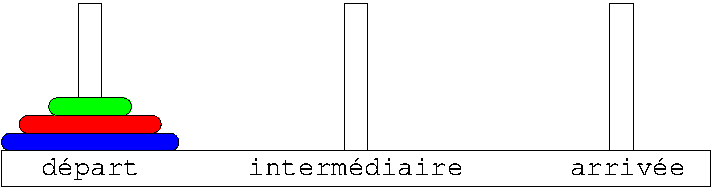
\includegraphics[width=6cm]{hanoi.pdf}}

{\bf Etat final :}\\
\centerline{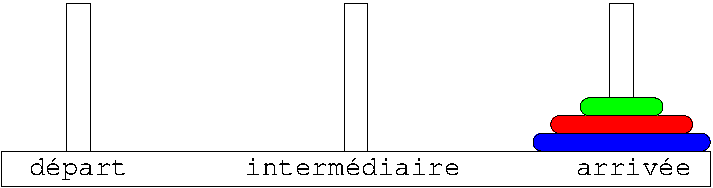
\includegraphics[width=6cm]{hanoi1.pdf}}
\end{minipage}}
}
Les « tours de Hanoï » est un jeu qui
consiste à déplacer $n$ disques de diamètres différents d'une 
tour de « départ » à une tour d'« arrivée » en passant par une 
tour « intermédiaire » et ceci en un minimum de coups, 
tout en respectant les règles suivantes :
\begin{itemize}
\item on ne peut déplacer qu'un disque à la fois,
\item on ne peut placer un disque que sur un autre disque 
	plus grand que lui ou sur une tour vide.
\end{itemize}
Dans l'état initial, les $n$ disques sont placés sur la tour
« départ ». Dans l'état final, tous les disques se retrouvent
placés dans le même ordre sur la tour « arrivéee ».

\index[algo]{tours de Hanoï}
\begin{lstlisting}[caption={\bf Tours de Hanoï},label=cl:hanoi]
def hanoi(n,gauche,milieu,droite):
    if n > 0:
        hanoi(n-1,gauche,droite,milieu)
        deplacer(n,gauche,droite)
        hanoi(n-1,milieu,droite,gauche)
    return
\end{lstlisting}
Si le déplacement se traduit par un simple affichage du type :
déplacer disque « n » de la tour «~gauche » à la tour « droite »,
alors l'appel de la procédure {\tt hanoi} pour $n = 3$ produit
les sorties suivantes.

\mbox{}\ \ \begin{py}{5cm}
\begin{verbatim}
def deplacer(n,gauche,droite):
    print 'déplacer disque', n,
          'de la tour', gauche, 
          'à la tour', droite
    return
\end{verbatim}
\end{py}
\hfill
\begin{py}{8cm}
\begin{verbatim}
>>> hanoi(3,'d','i','a')
déplacer disque 1 de la tour d à la tour a
déplacer disque 2 de la tour d à la tour i
déplacer disque 1 de la tour a à la tour i
déplacer disque 3 de la tour d à la tour a
déplacer disque 1 de la tour i à la tour d
déplacer disque 2 de la tour i à la tour a
déplacer disque 1 de la tour d à la tour a
\end{verbatim}
\end{py}
\vspace*{2mm}

%-------------------------------------------------------------------------
\section*{Tri bulles}\index{tri d'une séquence!tri bulles}
%-------------------------------------------------------------------------
\marginpar{\footnotesize\em
\begin{rem}Voir aussi le TD \ref{td:bulles} page \pageref{td:bulles}.
\end{rem}

\begin{rem} Le nom du tri bulles vient de ce que les éléments les plus petits 
(les plus « légers ») remontent vers le début de la liste comme des bulles vers le haut d'une
bouteille d'eau gazeuse.
\end{rem}
}

Dans le tri bulles, on parcourt la liste en commençant par la fin, en effectuant un échange à
chaque fois que l'on trouve deux éléments successifs qui ne sont pas dans le bon ordre.

%\newpage
\index[algo]{tri bulles}
\begin{lstlisting}[caption={\bf Tri bulles},label=cl:triBulles]
def triBulles(t,debut,fin):
    while debut < fin:
        for j in range(fin,debut,-1):
            if t[j] < t[j-1]: 
                t[j],t[j-1] = t[j-1],t[j]
        debut = debut + 1
    return t
\end{lstlisting}

\mbox{}\ \ \begin{py}{8cm}
\begin{verbatim}
>>> s = [9,8,7,6,5,4]
>>> triBulles(s,0,len(s)-1)
[4, 5, 6, 7, 8, 9]
\end{verbatim}
\end{py}
\hfill
\begin{py}{5cm}
\begin{verbatim}
>>> s = [9,8,7,6,5,4]
>>> triBulles(s,1,4)
[9, 5, 6, 7, 8, 4]
\end{verbatim}
\end{py}

%-------------------------------------------------------------------------
\section*{Tri fusion}\index{tri d'une séquence!tri fusion}
%-------------------------------------------------------------------------
Dans le tri fusion, on partage la liste à trier en deux sous-listes que l'on trie, et on
interclasse (on fusionne) ces deux sous-listes.

\newpage
\index[algo]{tri fusion}
\begin{lstlisting}[caption={\bf Tri fusion},label=cl:triFusion]
def triFusion(t,debut,fin):
    if debut < fin:
        m = (debut + fin)/2
        triFusion(t,debut,m)
        triFusion(t,m+1,fin)
        fusion(t,debut,m,fin)
    return t
\end{lstlisting}

La fusion consiste à construire, à partir des deux sous-listes triées (la première de
l'indice {\tt debut} à l'indice {\tt k}, la deuxième de l'indice {\tt k+1} à l'indice 
{\tt fin}) une liste elle-même triée des indices {\tt debut} à {\tt fin}
et contenant l'ensemble des éléments des deux sous-listes d'origine.

%\newpage
\begin{lstlisting}[title={\bf Fusion}]
def fusion(t,debut,k,fin):
    i1, i2 = debut, k+1
    while i1 <= k and i2 <= fin:
        if t[i2] >= t[i1]: i1 = i1 + 1
        else:
            t[i1], t[i1+1:i2+1] = t[i2], t[i1:i2]
            k = k + 1
            i2 = i2 + 1
    return t
\end{lstlisting}

\mbox{}\ \ \begin{py}{8cm}
\begin{verbatim}
>>> s = [4,5,6,1,2,3]
>>> fusion(s,0,2,len(s)-1)
[1, 2, 3, 4, 5, 6]
\end{verbatim}
\end{py}
\hfill
\begin{py}{5cm}
\begin{verbatim}
>>> s = [4,5,6,1,2,3]
>>> fusion(s,1,2,4)
[4, 1, 2, 5, 6, 3]
\end{verbatim}
\end{py}

%-------------------------------------------------------------------------
\section*{Tri par insertion}\index{tri d'une séquence!tri par insertion}
%-------------------------------------------------------------------------
\marginpar{\footnotesize\em
\begin{rem}
Voir aussi la section \ref{sub:triInsertion} page \pageref{sub:triInsertion} consacrée 
au tri par insertion.
\end{rem}
}

Dans le tri par insertion, on trie successivement les premiers éléments de la liste : à la
$i^{\grave eme}$ étape, on insère le $i^{\grave eme}$ élément à son rang parmi les $i-1$ éléments
précédents qui sont déjà triés entre eux.

\newpage
\index[algo]{tri par insertion}
\begin{lstlisting}[caption={\bf Tri par insertion},label=cl:triInsertion]
def triInsertion(t,debut,fin):
    assert type(t) is list
    assert 0 <= debut <= fin < len(t)
    for k in range(debut+1,fin+1):
        i = k - 1
        x = t[k]
        while i >= debut and t[i] > x:
            t[i+1] = t[i]
            i = i - 1
        t[i+1] = x
    return t
\end{lstlisting}

%-------------------------------------------------------------------------
\section*{Tri par sélection}\index{tri d'une séquence!tri par sélection}
%-------------------------------------------------------------------------
\marginpar{\footnotesize\em
\begin{rem}
Voir aussi la section \ref{sub:triSelection} page \pageref{sub:triSelection} consacrée 
au tri par sélection.
\end{rem}
}

Le tri par sélection d'une liste consiste à rechercher le minimum de la liste
à trier, de le mettre en début de liste en l'échangeant avec le premier élément
et de recommencer sur le reste de la liste.

\index[algo]{tri par sélection}
\begin{lstlisting}[caption={\bf Tri par sélection},label=cl:triSelection]
def triSelection(t,debut,fin):
    assert type(t) is list
    assert 0 <= debut <= fin < len(t)
    while debut < fin:
        mini = minimum(t,debut,fin)
        t[debut],t[mini] = t[mini],t[debut]
        debut = debut + 1
    return t
\end{lstlisting}

%-------------------------------------------------------------------------
\section*{Tri rapide}\index{tri d'une séquence!tri rapide}
%-------------------------------------------------------------------------
Le principe du tri rapide  est le suivant : on partage la 
liste à trier en deux sous-listes telles que tous les éléments de la première 
soient inférieurs à tous les éléments de la seconde.
Pour partager la liste en deux sous-listes, on choisit un des éléments de la liste
(par exemple le premier) comme pivot. On construit alors une sous-liste
avec tous les éléments inférieurs ou égaux à ce pivot et une sous-liste avec 
tous les éléments supérieurs au pivot.
On trie les deux sous-listes selon le même processus jusqu'à avoir des sous-listes 
réduites à un seul élément.
\marginpar{\footnotesize\em
\begin{rem}
Voir aussi la section \ref{sub:triRapide} page \pageref{sub:triRapide} consacrée 
au tri rapide.
\end{rem}
}

%\newpage
\index[algo]{tri rapide}
\begin{lstlisting}[caption={\bf Tri rapide},label=cl:triRapide]
def triRapide(t,debut,fin):
    assert type(t) is list
    assert 0 <= debut 
    assert fin <= len(t)
    if debut < fin:
        pivot = t[debut]
        place = partition(t,debut,fin,pivot)
        triRapide(t,debut,place-1)
        triRapide(t,place+1,fin)
    return t
\end{lstlisting}

\begin{lstlisting}[title={\bf Partition}]
def partition(t,debut,fin,pivot):
    place,inf,sup = debut,debut,fin;
    while place <= sup:
        if t[place] == pivot: place = place + 1
        elif t[place] < pivot:
            t[inf],t[place] = t[place],t[inf]
            inf = inf + 1
            place = place + 1
        else:
            t[sup],t[place] = t[place],t[sup]
            sup = sup - 1
    if place > 0: place = place - 1
    return place
\end{lstlisting}


\mbox{}\ \ \begin{py}{8cm}
\begin{verbatim}
>>> s = [3,6,5,4,1,2]
>>> partition(s,0,len(s)-1,4), s
(3, [3, 2, 1, 4, 5, 6])
\end{verbatim}
\end{py}
\hfill
\begin{py}{5cm}
\begin{verbatim}
>>> s = [3,6,5,4,1,2]
>>> partition(s,1,4,4), s
(2, [3, 1, 4, 5, 6, 2])
\end{verbatim}
\end{py}
